% siminos/reversal/Hill.tex      pdflatex LC21; bibtex LC21
% temporary: siminos/spatiotemp/chapter/LC21Hill.tex
% $Author: predrag $ $Date: 2021-12-24 01:25:20 -0500 (Fri, 24 Dec 2021) $

%\renewcommand{\Ssym}[1]{{\ensuremath{m_{#1}}}}
\renewcommand{\statesp}{state space}
\renewcommand{\Statesp}{State space}
\renewcommand{\stateDsp}{state-space}
\renewcommand{\StateDsp}{State-space}

\section{% Hill's formula:
         Stability of an orbit vs. its time-evolution stability}
\label{s:LC21Hill}
% PC started with: siminos/kittens/Hill.tex  2021-08-19

His 1878-1886 study of the stability of planar motion of the Moon around
the Earth led  Hill to the \emph{Hill's formula}\rf{Hill86}
\beq
\left|\Det\jMorb_c \right|= \left|\det (\id - \jMat_c)\right|
%\,.
\ee{detDet}
which relates the characteristic polynomial of the for\-ward-in-time
evolution {\po} Floquet matrix (monodromy matrix) $\jMat_c$ to the
determinant of the global {\jacobianOrb} $\jMorb_c$ (in Lagrangian
settings, the Hessian, the second variation of the action functional).
In case of Lagrangian dynamics, the discrete-time Hill's formula that we
use here was derived  by Mackay and Meiss\rf{MacMei83} in 1983.

Historically,  in \po\ theory calculations one always computes $\jMat_c$.
However, as we shall argue here, it is the {\HillDet} $\Det\jMorb_c$ that
is the computationally robust quantity that one should evaluate.
In his application Hill was lucky: $\Det\jMorb_c$ that he computed in a
$[3\!\times\!3]$ Fourier modes matrix approximation turned out to be a
quite good approximation.
But this is a remarkable formula, especially in the limit of
$\cl{}\to\infty$ infinitesimal time steps, a formula that relates the
$\infty$\dmn\ \emph{functional} {\HillDet} $\Det\jMorb_c$ to a
determinant of the finite $[d\!\times\!d]$ matrix $\jMat_c$, and it took
\Poincare\rf{Poinc1886} to prove that Hill's Fourier modes calculation is
correct in the continuum limit.

While first discovered in a Lagrangian setting, Hill's formulas are much
more general, with the Lagrangian formalism of
\refrefs{MacMei83,TreZub09,BolTre10,kooknewt} getting in the way of
understanding the general case.
The formula applies to dissipative dynamical systems as well, from the
Bernoulli map to \NS\ and \KSe\rf{GudorfThesis,GuBuCv17}. As the formula
is fundamental to the formulation of the \spt\ chaotic field theory, we
shall rederive it here in three ways, relying on nothing more than
elementary linear algebra.

The formula is so elementary that many practitioners routinely use it
without ever having heard of `Hill's formula'.
Let's say that a periodic $\ssp_{\zeit+\cl{}}=\ssp_\zeit$ {\lattstate}
$\Xx_c$ is known `numerically exactly', that is to say, to a high (but not
infinite) precision. One way to present the solution is to list the field
value $\ssp_0$ at a single lattice site $\zeit=0$, and let the reader
reconstruct the rest by stepping forward in time,
$\ssp_{\zeit}=\hat{\map}^\zeit(\ssp_0)$.

However, for a linearly unstable orbit a single  field value $\ssp_0$
does not suffice to present the solution, because there is always a finite
`Lyapunov time' $\zeit_{Lyap}$  beyond which $\hat{\map}^\zeit(\ssp_0)$
has lost all memory of the {\lattstate} $\Xx_c$. This problem is particularly
severe in searches for {`\ecs s'} embedded in turbulence, where even the
shortest period solutions have to be computed to the (for a working fluid
dynamicist excessive) machine
precision\rf{GHCW07,channelflow,openpipeflow}, in order to complete the
first return to the initial state. So, the words uttered in introductory
nonlinear dynamics courses is never what is practiced.

Instead of relaying on for\-ward-in-time numerical integration,
\emph{global methods} for finding periodic orbits\rf{ChoGuck99} view them
as equations for the vector fields $\dot{\ssp}$ on spaces of closed
curves. In numerical implementations one discretizes a \po\  $p$ into
sufficiently many short
segments\rf{auto,GM00aut,ChoGuck99,DingCvit14,DCTSCD14}, and lists one
field value for each segment
\beq
p=(\ssp_1,\ssp_2,\cdots,\ssp_\cl{c})
\,.
\ee{discrOrbit}
For a $\cl{c}$\dmn\ discrete time map $\hat{\map}$ obtained by cutting the flow by
$\cl{c}$ local {\PoincSec s}, with the \po\ $c$ of discrete period $\cl{c}$,
every segment can be reconstructed by short time integration, and
satisfies
\beq
\ssp_{\zeit+1}=\hat{\map}_\zeit(\ssp_\zeit)
\,,
\ee{CyclePntErr}
to high accuracy, as for sufficiently short times the exponential
instabilities are numerically controllable.

% PC 2021-10-23
%     moved from siminos/spatiotemp/chapter/LC21Bernoulli.tex
\subsection{{\HillDet} for a $d$-component lattice field}
\label{s:LC21notHill}   % was {exam:Hill1stOrd}
% maybe call this {Hill's formula for a general first-order system}
% siminos/spatiotemp/Examples/examHill1stOrd.tex

The {\jacobianOrb} $\jMorb_{\zeit\zeit'}$ \refeq{jacobianOrb} is a
high-\dmn\ linear stability matrix for the extremum condition
$F[\Xx_c]=0$, evaluated on the {\lattstate} $\Xx_c$. How is the stability
so computed related to the conventional dynamical systems'
for\-ward-in-time stability? To motivate the answer in its generality,
consider a temporal lattice with a set of $d$ fields
$\ssp_{\zeit}=\{\ssp_{\zeit,1},\ssp_{\zeit,2},\dots,\ssp_{\zeit,d}\}$ on
each lattice site $\zeit$, and time evolution given by a $d$\dmn\ map
$\ssp_{\zeit+1}=\hat{\map}(\ssp_{\zeit})$.
A period-$\cl{}$ {\lattstate} \refeq{pathBern} thus
satisfies site-by-site the first-order difference equation
\beq
\ssp_{\zeit} - \hat{\map}(\ssp_{\zeit-1}) = 0
    \,,\qquad
\zeit=1,2,\cdots,\cl{}
\,.
\ee{1stepNonlimTemp}
A small deviation $\Delta\Xx$ from $\Xx_p$ then satisfies the linearized condition
\beq
\Delta\ssp_{\zeit} - \shift^{-1}\jMat_{\zeit}\,\Delta\ssp_{\zeit} = 0
\,,\qquad
(\jMat_{\zeit})_{ij}
=
        %\left.
        \frac{\partial \flow{}{\ssp_\zeit}_i }
             {\partial \ssp_j                }
        %\right|_{\ssp_{j}=\ssp_{\zeit,j}}
\,,
\ee{d-1stepJac2}
where $\jMat_{\zeit}$ is the 1-time step $[d\!\times\!{d}]$
\jacobianM, evaluated on lattice site $\zeit$.

It suffices to work out a temporal period $\cl{}=3$ example to understand
the calculation for any period. In terms of the $[3d\!\times\!3d]$
generalized \refeq{hopMatrix} block shift matrix $\shift$, the \jacobianOrb\
\refeq{jacobianOrb} has block matrix form
\beq
\jMorb_p \,=\,
\id-\shift^{-1}\jMat
\,,\quad
\shift =
\left[
\begin{array}{ccc}
0     & \id_d& 0   \\
0     & 0     & \id_d\\
\id_d& 0     & 0
\end{array}
\right]
\,,\quad
\jMat =
\left[
\begin{array}{ccc}
\jMat_1 & 0 & 0 \\
0 & \jMat_2 & 0  \\
0 & 0 & \jMat_3
\end{array}
\right]
\,,
\ee{3shift}
where $\id  $ is the $d$\dmn\ identity matrix.
Next, consider
\beq
\shift^{-1}\jMat =
\left[
\begin{array}{ccc}
0       & 0       & \jMat_3   \\
\jMat_1 & 0       & 0  \\
0       & \jMat_2 & 0
\end{array}
\right]
,\;\;
(\shift^{-1}\jMat)^2 \,=\,
\left[
\begin{array}{ccc}
0 & \jMat_3\jMat_2 & 0 \\
0 & 0 & \jMat_1\jMat_3  \\
\jMat_2\jMat_1 & 0 & 0
\end{array}
\right]
\,,
\ee{stabShift}
and note that the $\cl{}=3$ repeat of $\shift^{-1}\jMat$ is block-diagonal
\bea
(\shift^{-1}\jMat)^3  =
\left[
\begin{array}{ccc}
\jMat_3\jMat_2\jMat_1 & 0 & 0 \\
0 & \jMat_1\jMat_3\jMat_2 & 0  \\
0 & 0 & \jMat_2\jMat_1\jMat_3
\end{array}
\right]
\,,
\label{stabCube}
\eea
with $[d\!\times\!{d}]$ blocks cyclic permutations of each other.f
In general, % as $\shift^\cl{}=\id$,
the trace of the
$[\cl{}d\!\times\!\cl{}d]$ matrix for a period $\cl{}$ {\lattstate}
\[
\Tr(\shift^{-1}\jMat)^k=\delta_{k,r\cl{}}\,\cl{}\,\tr\jMat_p^r
\,,\quad
\jMat_p = \jMat_\cl{}\jMat_{\cl{}-1}\cdots\jMat_2\jMat_1
\]
is non-vanishing only if $k$ is a multiple of $\cl{}$, where $\jMat_p$ is the
for\-ward-in-time $[d\!\times\!{d}]$ Floquet matrix of the \po\ $p$.

Now we can evaluate the {\HillDet}
$\Det\jMorb_p$ by expanding
\bea
\ln\Det\jMorb_p &=&
\Tr\ln(\id-{\shift}^{-1}\jMat)
                \,=\,
-\sum_{k=1}^\infty\frac{1}{k}\,\Tr({\shift}^{-1}\jMat)^k
    \continue
                 &=&
-\tr\sum_{r=1}^\infty\frac{1}{r} \jMat_p^{r}
  =
\ln\det(\id_d-\jMat_p)
\,.
\label{LnDet=TrLn2}
\eea
The {\jacobianOrb} $\jMorb_p$ evaluated on a {\lattstate} $\Xx_p$
satisfying the temporal lattice first-order difference equation
\refeq{1stepNonlimTemp}, and the dynamical, for\-ward-in-time \jacobianM\
$\jMat_p$ are thus related by \emph{Hill's formula}
\beq
\Det\jMorb_p = \det(\id  -\jMat_p)
\,,
\ee{detDet}
which relates the global orbit stability to the Floquet, for\-ward-in-time
evolution stability.

As far as the time-evolution stability is concerned, the
$|\Det\jMorb_\Mm|=|\det (\id-\jMat_\Mm)|$ formula \refeq{detDet} is
correct for all first-order difference equations (systems whose evolution
laws are first order in time), for any $[d\times{d}]$ one-time-step
{\jacobianM}. For the Bernoulli system that is a $[1\!\times\!1]$ matrix
$\jMat=s$, with the periodic points count \refeq{detBern2} trivially
verified.

The temporal {Bernoulli} \refeq{tempBern} is a particularly simple, linear  example.
The site field $\ssp_\zeit$ is a scalar,
the 1-time step $[1\!\times\!1]$ time-evolution \jacobianM\
\refeq{d-1stepJac2} at every lattice point $\zeit$ is simply
$\jMat_{\zeit}={s}$,
and
the {\jacobianOrb}
\refeq{tempBern} is the same for all {\lattstate}s of period $\cl{}$,
so
\beq
\mbox{temporal {Bernoulli}: }\quad
N_\cl{} = |\Det\jMorb| = {s}^{\cl{}} - 1
\,,
\ee{LC21detBern}
in agreement with the time-evolution count \refeq{noPerPtsBm}; all
itineraries are allowed, except that the periodicity of
$\shift^\cl{}=\id$ accounts for $\cycle{0}$ and
$\cycle{s\!-\!1}$ fixed points (see \reffig{fig:BernPart}) being a
single periodic point.



\subsection{{\HillDet} of a for\-ward-in-time map}
\label{s:LC21forwardHill}

For a $d$\dmn\ deterministic map $\ssp_{\zeit+1} = \hat{\map}(\ssp_{\zeit})$, the
{\FPoper}
\beq
     \Lop\,\msr(\ssp_{\zeit+1})
= \int_\pS\!\! d\ssp_{\zeit}\,
           \delta(\ssp_{\zeit+1} - \hat{\map}(\ssp_{\zeit}))\,
           \msr(\ssp_{\zeit})
%\,,
\ee{PerronFrobenius}
maps a density distribution $\msr(\ssp_{\zeit})$ for\-ward-in-time.
Its kernel, a $d$\dmn\ Dirac delta function
\bea
\Lop(\ssp_{\zeit+1},\ssp_{\zeit})
    = \delta(\ssp_{\zeit+1} - \hat{\map}(\ssp_{\zeit}))
\,,
\eea
applied repeatedly, satisfies the group property
\beq
\Lop^2(\ssp_{\zeit+2},\ssp_{\zeit})
    = \int_\pS\!\! d\ssp_{\zeit+1}\,
            \Lop(\ssp_{\zeit+2},\ssp_{\zeit+1})\,
            \Lop(\ssp_{\zeit+1},\ssp_{\zeit})
    = \delta(\ssp_{\zeit+2}-\flow{2}{\ssp_{\zeit}})
\,.
\ee{FPsemiGroup}
The time-evolution periodic orbit theory\rf{ChaosBook} relates the
long time chaotic averages to the traces of the {\FPoper}
\beq
\tr\Lop^\cl{}
     = \int_\pS\!\!d\ssp\,\Lop^\cl{}(\ssp,\ssp)
     = \int_\pS\!\!d\ssp_{c}\,\delta(\ssp_{c} - \flow{\cl{}}{\ssp_c})
\eeq
and its weighted, evolution operator generalizations, with support on all
periodic points / {\lattstate}s   $\ssp_{c}=\flow{\cl{}}{\ssp_c}$ of
period $cl{}$.

To evaluate the trace of the $\cl{}$th iterate of the {\FPoper},
one can either use the kernel of the operator
$\Lop^\cl{}(\ssp_{\cl{}},\ssp_0) = \delta(\ssp_{\cl{}} - \flow{\cl{}}{\ssp_0})$,
\bea
\tr \Lop^\cl{} &=&  \int_\pS\!\!d\ssp_0 \, \delta(\ssp_{0}-\flow{\cl{}}{\ssp_0})
\,,
\eea
or, using the group property \refeq{FPsemiGroup} to insert integrations
over intermediate lattice sites, the product of one-time-step operators $\Lop$:
\bea
\tr \Lop^\cl{} &=&
\int  d\Xx \prod_{\zeit=0}^{\cl{}-1} \delta(\ssp_{\zeit+1}-\hat{\map}(\ssp_{\zeit})) \,,
\continue
\ssp_{\cl{}} &=& \ssp_0 \,, \quad d\Xx
              = \prod_{\zeit=0}^{\cl{}-1} d \ssp_{\zeit}
\,.
\label{PerronFrobeniusTrace}
\eea
The field $\ssp_{\zeit}$ on every lattice site $\zeit$ is a $d$\dmn\
vector, so a period-\cl{} {\lattstate} \Xx\ is a $\cl{}d$\dmn\ vector,
with the Dirac function also $\cl{}d$\dmn. In matrix notation this trace
takes a compact form:
\bea
\tr \Lop^\cl{} = \int d\Xx\,\delta(\shift \Xx - \hat{\map}(\Xx)) \,,
\eea
where $\Xx$ and $\hat{\map}(\Xx)$ are $\cl{}d$\dmn\ column vectors with
$(id+j)$th components $(\ssp_{\zeit})_j$ and
$[\hat{\map}(\ssp_{\zeit})]_j$, where $0 \leq i < \cl{}-1$, $0 \leq j < d-1$,
and $\shift$ is the cyclic $[\cl{}d\!\times\!\cl{}d]$ {\shiftOp}
(compare with \refeq{hopMatrix}):
\beq
\shift
=  \left(\begin{array}{ccccc}
             0    &  \id      &        &   &  \cr
                  &  0    &   \id      &   &  \cr
                  &       &        & \ddots &  \cr
                  &       &        & 0 & \id   \cr
             \id      &       &        &   & 0
          \end{array} \right)
\,,
\eeq
where $\id  $ is the $d$\dmn\ identity matrix.
Note that the vector
in the $\cl{}d$\dmn\ Dirac delta function is the defining equation
\refeq{LC21eqMotion} of the system:
\[
F[\Xx] = \shift \Xx - \hat{\map}(\Xx) \,.
\]

\refeq{LC21eqMotion}
with a global deterministic solution $\Xx_c$ satisfying this local extremal
condition on every lattice site.


Restricting the integration to an infinitesimal neighborhood
$\pS_p$ around a periodic point $\ssp_p$, the contribution from this periodic point is:
\bea
\tr\left.\Lop^\cl{}\right|_p =
       \int_{\pS_p} \!\!d\ssp_0\,\delta(\ssp_{0}-\flow{\cl{}}{\ssp_0})
       =\frac{1}{\left|\det(\id - \jMat_p)\right|} \,,
\label{ForwardInTimeTr}
\eea
where $\jMat_p$ is the $[d\!\times\!d]$ for\-ward-in-time Floquet matrix of
the periodic orbit \refeq{d-1stepJac2} started from the periodic point
$\ssp_p$ with period $\cl{}$. Compute the trace using the integral on
$\cl{}$ points:
\bea
\tr_p \Lop^\cl{} &=&
\int_{\pS_p}\!\!d\Xx\,\prod_{i=0}^{\cl{}-1}
            \delta(\ssp_{\zeit+1}-\hat{\map}(\ssp_{\zeit}))
                  = \int_{\pS_{p}}\!\!\!d\Xx\,\delta(F[\Xx])
\continue
&=& \frac{1}{\left|\Det\jMorb_p\right|}
\,,
\label{GlobalTr}
\eea
where
\bea
\jMorb_p = \frac{\partial F[\Xx]}{\partial \Xx}
\eea
is the $[\cl{}d\!\times\!\cl{}d]$ {\jacobianOrb} of the period-$\cl{}$
{\lattstate} started with $\ssp_p$.
$\pS_{p}$ is a region in the $\cl{}d$\dmn\ \statesp\ of $\Xx$ whose first
$d$ components are the infinitesimal neighborhood around $\ssp_p$.
Comparing the trace \refeq{ForwardInTimeTr} and \refeq{GlobalTr}, we have
proved the Hill's formula \refeq{detDet}.

\subsection{{\HillDet} for a 2nd order difference equation}
\label{s:LC21Hill2step}

An $n$-step recurrence relation is the discrete-time analogue of an $n$th
order differential equation. In formulating dynamical systems problems,
one almost always replaces higher order derivatives (Euler-Lagrange
equations) by sets of fields satisfying first order equations (Hamilton's
equations), and the same is true for discrete time systems. For example,
the Hamiltonian \templatt\ and \HenonMap\ are usually formulated as
time-evolution over a 2\dmn\ phase space \refeq{catMap} and
\refeq{LC21eq2.1}, rather than the 3-term recurrence configuration space
conditions \refeq{catMapNewt} and \refeq{LC21:2-step}.

A $k$th order differential equation can be discretized as a $k$th order
difference equation. Just as a scalar field satisfying a $k$th order
differential equation can be replaced by a set of $k$ fields, each
satisfying a first order equation, a $k$th order difference equation for
a scalar field can be replaced by a $k$\dmn\ vector field, satisfying $k$
$1$st order difference equations.

One can compute the orbit stability of a scalar field {\lattstate} of
such system using the for\-ward-in-time Hill's formula for the $k$\dmn\
vector field representation of dynamics, and the corresponding the
determinant of the $[k\cl{} \times k\cl{}]$ {\jacobianOrb}
\refeq{GlobalTr}. However, with the recurrence relation, the
{\jacobianOrb} has a simpler form.

Consider a map with a 3-term recurrence relation, $\ssp_{\zeit+1} = \map(\ssp_{\zeit-1}, \ssp_{\zeit})$,
where $\ssp_{\zeit-1}$, $\ssp_{\zeit}$ and $\ssp_{\zeit+1}$ are scalars.
This map can be replaced by a pair of 1st order difference equations
$(\ssp_{\zeit}, \ssp_{\zeit+1}) = \hat{f}(\ssp_{\zeit-1}, \ssp_{\zeit}) = (\ssp_{\zeit}, \map(\ssp_{\zeit-1},\ssp_{\zeit}))$.
The trace of the $\cl{}$th iterate of the {\FPoper} can be
evaluated using the Dirac delta kernel of the operator $\Lop^\cl{}$, or the
product of $\Lop$ and the recurrence relation:
\bea
\tr \Lop^\cl{} &=&  \int d \ssp_0 d \ssp_1 \delta((\ssp_{0},\ssp_1) -
\hat{f}^\cl{}(\ssp_0,\ssp_1))
\continue
               &=&
\int [d \Xx] \prod_{i=0}^{\cl{}-1} \delta(\ssp_{\zeit+1}-\map(\ssp_{\zeit-1},\ssp_{\zeit})) \,,
\continue
\ssp_{\cl{}} &=& \ssp_0 \,, \quad
\ssp_{-1} = \ssp_{\cl{}-1} \,, \quad
[d \Xx] = \prod_{i=0}^{\cl{}-1} d \ssp_{\zeit} \,.
\eea
Using the matrix notation, the trace computed by
the integral on $\cl{}$ points along a discrete periodic orbit is:
\bea
\tr \Lop^\cl{} = \int [d \Xx] \delta(\shift \Xx - \map(\shift^{-1} \Xx, \Xx)) \,,
\eea
where $\Xx$ and $\map(\shift^{-1} \Xx, \Xx)$ are $\cl{}$\dmn\ column vectors with $i$th components
$\ssp_{\zeit}$ and $\map((\shift^{-1}\Xx)_i,\Xx_i)$, and $\shift$ is the cyclic $[\cl{}\!\times\! \cl{}]$
{\shiftOp} \refeq{hopMatrix}. The vector in the Dirac delta function is the defining equation of
the system:
\bea
F[\Xx] = \shift \Xx - \map(\shift^{-1} \Xx, \Xx) \,.
\eea
Restricting the integration to an infinitesimal neighborhood
$\pS_p$ around a periodic point $(\ssp_{p,0},\ssp_{p,1})$ with period $\cl{}$,
the contribution from this periodic point is:
\bea
\tr_p \Lop^\cl{} = \int_{\pS_p} d \ssp_0 d \ssp_1 \delta((\ssp_{0},\ssp_1) -
\hat{f}^\cl{}(\ssp_0,\ssp_1))
=\frac{1}{\left|\det(\id - \jMat_p)\right|} \,,
\label{ForwardInTimeTrRecurrence}
\eea
where
\bea
\jMat_p = \frac{\partial \hat{f}^{\cl{}}(\ssp_{p,0},\ssp_{p,1})}{\partial (\ssp_{p,0},\ssp_{p,1})}
\eea
is the $[2\!\times\!2]$ for\-ward-in-time Floquet matrix of the periodic orbit
started from the periodic point
$(\ssp_{p,0},\ssp_{p,1})$ with period $\cl{}$. Compute the trace using the
integral on $\cl{}$ points:
\bea
\tr_p \Lop^\cl{} &=&
\int_{\pS_{\Xx_p}} [d \Xx] \delta(\shift \Xx - \map(\shift^{-1} \Xx, \Xx))
                  = \int_{\pS_{\Xx_p}} [d \Xx] \delta(F[\Xx])
\continue
                 &=& \frac{1}{\left|\Det\jMorb_p\right|}
\,,
\label{GlobalTrRecurrence}
\eea
where
\bea
\jMorb_p = \frac{\partial F[\Xx_p]}{\partial \Xx_p}
\eea
is the $[\cl{}\!\times\!\cl{}]$
{\jacobianOrb} of the period-$\cl{}$ {\lattstate} started with $(\ssp_{p,0},\ssp_{p,1})$.
$\pS_{\Xx_p}$ is a region in the $\cl{}$\dmn\ space of $\Xx$ whose first 2
components are the infinitesimal neighborhood around $(\ssp_{p,0},\ssp_{p,1})$.
Compare the trace \refeq{ForwardInTimeTrRecurrence} and
\refeq{GlobalTrRecurrence}, we have proved the Hill's formula \refeq{detDet}.

\HL{2021-12-16}{The rest of this section is from the old version.
        }

Our task is to compute the {\HillDet} $|\det \jMorb|$. We first show how
to do that directly, by computing the volume of the {\fundPip}.

\subsection{{\HillDet}: fundamental parallelepiped evaluation}
\label{s:LC21fundFacteval}
% 2020-02-16 Predrag computed  using siminos/mathematica/Tensors.nb
As a concrete example
consider the Bravais lattice % \refeq{1DBravLatt}
with basis
vector

The {\em \jacobianOrb} is the $\delta/\delta\ssp_k$ derivative of the
{\henlatt} 3-term recurrence relation \refeq{jMorb1dFT}
\bea
\jMorb_p &=& - \shift + 2\,{\mathbb{X}}_p - \shift^{-1}
\,,
\label{Henlatt-orbitJac}
\eea
where ${\mathbb{X}}_p$ is a diagonal matrix with $p$-{\lattstate} $\ssp_k$ in the
$k$th row/column, and the `$1$'s in the upper right and lower left corners
enforce the periodic boundary conditions.

The action of the \henlatt\ {\jacobianOrb} can be hard to visualize,
as a period-2 {\lattstate} is a 2-torus,
period-3 {\lattstate} a 3-torus, \etc. Still, the {\fundPip} for the period-2
and period-3 {\lattstate}s, should suffice to
convey the idea. The {\fundPip} basis vectors \refeq{lattJac} are the
columns of $\jMorb$. The $[2\!\times\!2]$ {\jacobianOrb}
and its {\HillDet} follow from \refeq{Henlatt-2-cycle}
\beq
\jMorb =
 \left(\begin{array}{cc}
2\,\ssp_0   & -2 \\
         -2 & 2\,\ssp_1
 \end{array} \right)
\,,\quad
\Det\jMorb = 4\,(\ssp_0\ssp_1-1)
           = -4\,(a-3)
\,.
\ee{Henlatt-catFundPar2}
% $( 1+ \sqrt{a-3} )( 1- \sqrt{a-3} )-1 = -a+3$
The resulting {\fundPip} shown in \reffig{fig:Henlatt-catCycJacob}\,(a).
Period-3
{\lattstate}s for $s=3$ are contained in the half-open {\fundPip} of
\reffig{fig:Henlatt-catCycJacob}\,(b),
defined by the columns of $[3\!\times\!3]$
{\jacobianOrb}
\beq
\jMorb =
\left(
\begin{array}{ccc}
2\,\ssp_0 &-1           &-1 \\
         -1 & 2\,\ssp_1 &-1 \\
         -1 &-1           & 2\,\ssp_2
\end{array}
\right)
\,,
\qquad
\Det \jMorb
    = 8\,\ssp_0\ssp_1\ssp_2-2\,(\ssp_0+\ssp_2+\ssp_3)+2
\,,
\label{Henlatt-catFundPar3}
\eeq

\subsection{Fundamental fact} %{Integer lattices}
\label{sect:fundFact}

The {\jacobianOrb} \jMorb\ stretches the \statesp\ unit hyper-cube
$\Xx\in[0,1)^\cl{}$ into the \cl{}\dmn\ {\em \fundPip}, and maps each
periodic point ${\Xx}_{\Mm}$ into an integer lattice $\integers^\cl{}$
site, which is then translated by the winding numbers $\Mm$ into the
origin, in order to satisfy the fixed point condition
\refeq{tempFixPoint}. Hence $N_\cl{}$, the total number of the solutions
of the fixed point condition equals the number of integer lattice points
within the {\fundPip}, a number given by what Baake \etal\rf{BaHePl97}
call the \emph{`fundamental fact'},
\beq
N_\cl{} = |\Det\jMorb|
\,,
\ee{fundFact}
\ie, fact that the number of integer points in the {\fundPip} is equal to
its volume, or, what we refer to as the `{\HillDet}' below. In two
dimensions this formula is known since 1899 as
\HREF{https://en.wikipedia.org/wiki/Pick\%27s_theorem} {Pick's theorem},
in higher dimensions it was given by Nielsen\rf{Nielsen1920,BBPT75} in
1920, and rederived several times since in different contexts, for
example by Baake \etal\rf{BaHePl97}. For the task at hand,
Barvinok\rf{Barvinok04}
\HREF{http://www.math.lsa.umich.edu/~barvinok/lectures.pdf} {lectures}
offer a clear and simple introduction to integer lattices, and a proof of
\refeq{fundFact}.
% as {theorem 2}.

%%%%%%%%%%%%%%%%%%%%%%%%%%%%%%%%%%%%%%%%%%%%%%%%%%%%%%%%%%%%%%%%%%%%%%%
% BernCyc2Jacob.svg
% derived from CatMapStatesp.svg
\begin{figure}
  \centering
(a)~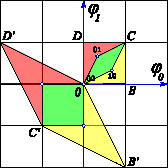
\includegraphics[width=0.35\textwidth]{BernCyc2JacobUnit}
~~~~~~
(b)~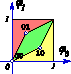
\includegraphics[width=0.22\textwidth]{BernCyc2JacobPart}
  \caption{\label{fig:BernCyc2Jacob}
(Color online)~~~
  (a)
The Bernoulli map \refeq{BerShift} periodic points
$\Xx_\Mm=(\ssp_0,\ssp_1)$ of period 2 are the $\cycle{0}=(0,0)$ fixed
point, and the 2-cycle $\Xx_{01}=({1}/{3},{2}/{3})$, see
\reffig{fig:BernPart}\,(a). They all lie within the unit square $[0BCD]$,
which is mapped by the {\jacobianOrb} $\jMorb$ \refeq{bernFundPar} into
the {\fundPip} $[0B'C'D']$. Periodic points $\Xx_\Mm$ are mapped by
$\jMorb$ onto the integer lattice, $\jMorb\Xx_\Mm\in\integers^\cl{}$, and
are sent back into the origin by integer translations $\Mm$, in order to
satisfy the fixed point condition \refeq{tempFixPoint}. Note that this
{\fundPip} is covered by  3 unit area quadrilaterals, hence
$|\Det\jMorb|=3$.
    (b)
Conversely, in the flow conservation sum rule \refeq{H-OdeA_mapsOrb2} sum
over all {\lattstate}s $\Mm$ of period $\cl{}$, the inverse of the
{\HillDet} defines the `neighborhood' of a lattices state as the
corresponding fraction of the unit hypercube volume.
          }
\end{figure}
%%%%%%%%%%%%%%%%%%%%%%%%%%%%%%%%%%%%%%%%%%%%%%%%%%%%%%%%%%%%%%
%
The action of {\jacobianOrb}
$\jMorb$ for the period-2 {\lattstate}s (periodic points) of the Bernoulli map of
\reffig{fig:BernPart}\,(a), suffices to convey the idea. In this
case, the $[2\!\times\!2]$ {\jacobianOrb} \refeq{tempBern}, the unit
square basis vectors, and their images are
\bea
\jMorb &=&
 \left(\begin{array}{cc}
  2 & -1 \\
 -1 &  2
 \end{array} \right)
    \continue
\Xx^{(B)} &=&
 \left(\begin{array}{c}
 1  \\
 0
 \end{array} \right)
\;\to\;
\Xx^{(B')} = \jMorb\,\Xx^{(B)} =
 \left(\begin{array}{c}
  2  \\
 -1
 \end{array} \right)
\,,\quad \cdots
\nnu
\eea
\ie, the columns of the {\jacobianOrb} are the edges of the {\fundPip},
\beq
\jMorb = \left(\Xx^{(B')}\Xx^{(D')}\right)
\,,
\ee{bernFundPar}
see \reffig{fig:BernCyc2Jacob}\,(a), and $N_2=|\Det\jMorb|=3$,
in agreement with the periodic orbit count \refeq{noPerPtsBm}.

In general, the unit vectors of the \statesp\ unit hyper-cube
$\Xx\in[0,1)^\cl{}$ point along the \cl{} axes; {\jacobianOrb} \jMorb\
stretches them into a {\fundPip} basis vectors $\Xx^{(j)}$, each one a
column of the $[\cl{}\!\times\!\cl{}]$ matrix
\beq
\jMorb = \left(\Xx^{(1)}\Xx^{(2)}\cdots\Xx^{(\cl{})}\right)
\,.
\ee{lattJac}
The {\HillDet}
\beq
\Det \jMorb = \Det\!\left(\Xx^{(1)}\Xx^{(2)}\cdots\Xx^{(\cl{})}\right)
\,,
\ee{lattVol}
is then the volume of the {\fundPip} whose edges are basis vectors
$\Xx^{(j)}$. Note that the unit hypercubes and {\fundPip}s are half-open,
as indicated by dashed lines in \reffig{fig:BernCyc2Jacob}\,(a), so that
their translates form a partition of the extended \statesp\
\refeq{BerStretch}. For another example of {\fundPip}s, see
\reffig{fig:catCycJacob}.
% and \refeq{3times2basisVecs}.

Note that in the {temporal lattice} reformulation, the Bernoulli system
involves two distinct lattices:
\begin{itemize}
  \item[(i)]
Any lattice field theory:
in the discretization \refeq{LattField}
 of the time continuum, one replaces \emph{any}
dynamical system's time-dependent field $\ssp(\zeit)\in\reals$ at time
$\zeit\in\reals$ by a discrete set of its values
$\ssp_\zeit=\ssp(a\,\zeit)$ at time instants $\zeit\in\integers$.
Here the index $\zeit$ is a \emph{coordinate} over which the field
$\ssp$ is defined.
  \item[(ii)]
Specific to the Bernoulli system: the site $\zeit$ field value
$\ssp_{\zeit}$ \refeq{n-tuplingMap} is confined to the unit interval
$[0,1)$, imparting integer lattice structure onto the intermediate
calculational steps in the extended \statesp\ \refeq{BerStretch} on which
the {\jacobianOrb} \jMorb\ \refeq{tempBern} acts.
\end{itemize}

    \PC{2021-10-25}{
    Combine the above with the \templatt\ \refpage{} discussion into a
    remark that temporal Bernoulli and \templatt\ aslo have a
    \emph{dynamical} \Dn{1} symmetry, not utilized in this paper, as
    nonlinear field theories such as \henlatt\ do not have such
    symmetries. Here we study only the symmetries of the floor, not the
    dancer.
    }

For \templatt\ the total number of {\lattstate}s is again, as
for the Bernoulli system \refeq{fundFact}, given by the `fundamental
fact \refeq{fundFact}.
However, while for the temporal Bernoulli every sequence of alphabet
letters \refeq{base-sAlph}  but one is admissible, for \templatt\ the
condition \refeq{catMapNewt} constrains admissible source {\brick}s \Mm.

For period-1, constant field  {\lattstate}s
$\ssp_{\zeit+1}=\ssp_{\zeit}=\ssp_{\zeit-1}$
it follows from
\refeq{catMapNewt} that
\[
        ({s}-2)\ssp_\zeit = \Ssym{\zeit}
\,,
\]
so the {\jacobianOrb} is a $[1\times1]$ matrix, and there are
\beq
N_1={s}-2
%\,,
\ee{catFundPar1}
period-1 {\lattstate}s. This is easy to verify by counting the admissible
$\Ssym{\zeit}$ values. Since $\ssp_\zeit \in [0,1)$, the range of
\Ssym{\zeit} is $\Ssym{\zeit} \in [0,s-2)$. So three of the
\refeq{catAlphabet}  \templatt\  letters are not admissible:
$\underline{1}$ is below the range, and $s-2$ and $s-1$ are above it.

%%%%%%%%%%%%%%%%%%%%%%%%%%%%%%%%%%%%%%%%%%%%%%%%%%%%%%%%%%%%%
% Predrag 2020-02-08 replaced Han's
% {HLLength2Counting}.pdf by hand-drawn catCyc2Jacob.svg
% Han & PC 2020-02-11
% siminos/figSrc/han/Mathematica/CountingFigure/HLLength3Counting.nb
\begin{figure}
  \centering
(a)~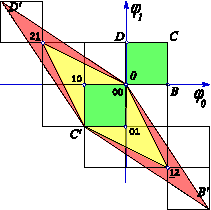
\includegraphics[width=0.38\textwidth]{catCyc2JacobUnit}
~~~
(b)~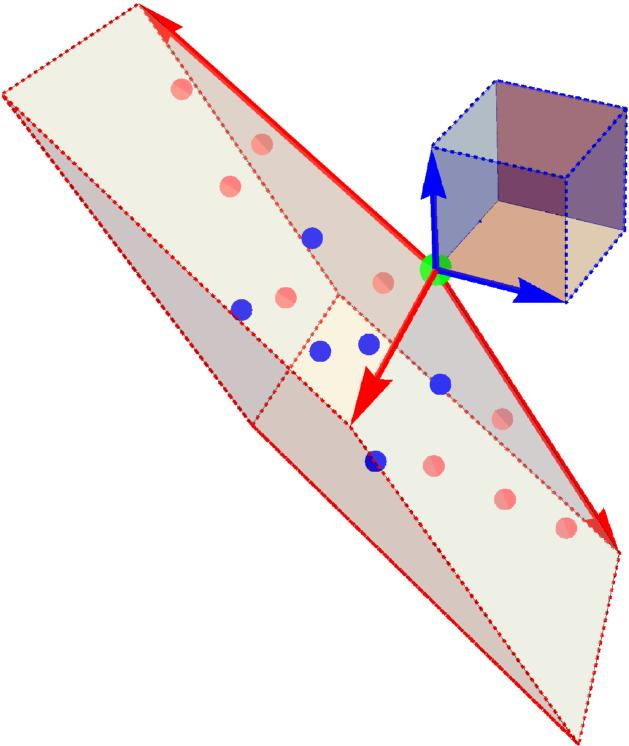
\includegraphics[width=0.34\textwidth]{PCLength3Counting}
  \caption{\label{fig:catCycJacob}
    (Color online)~~~
(a)
    For $s=3$, the \templatt\ \refeq{catTempLatt} has 5 period-2
    {\lattstate}s $\Xx_\Mm=(\ssp_0,\ssp_1)$: $\Xx_{00}$ fixed point and
    2-cycles $\{\Xx_{01},\Xx_{10}\}$,
    $\{\Xx_{\underline{1}2},\Xx_{2\underline{1}}\}$. They lie
    within the unit square $[0BCD]$, and are mapped by the
    $[2\!\times\!2]$ {\jacobianOrb} $\jMorb$ \refeq{catFundPar2} into the
    {\fundPip} $[0B'C'D']$, as in, for example, Bernoulli
    \reffig{fig:BernCyc2Jacob}. The images of periodic points $\Xx_\Mm$
    land on the integer lattice, and are sent back into the origin by
    integer translations $\Mm= \Ssym{0}\Ssym{1}$, in order to satisfy the
    fixed point condition
    %\refeq{tempFixPoint},
    $\jMorb\Xx_\Mm+\Mm=0$.
(b) A 3-dimensional [{\color{blue} blue} basis vectors] unit-cube stretched by
    $\jMorb$ \refeq{catFundPar3} into the [{\color{red} red} basis vectors]
    {\fundPip}. For $s=3$, the \templatt\
    \refeq{catTempLatt} has 16 period-3 {\lattstate}s: a $\Xx_{000}$
    fixed point at the vertex at the origin, [{\color{red} pink dots}] 3
    period-3 orbits on the faces of the {\fundPip}, and
    [{\color{blue} blue dots}] 2 period-3 orbits in its interior.
    An \cl{}\dmn\ \statesp\ unit hyper-cube $\Xx\in[0,1)^\cl{}$ and the
    corresponding {\fundPip} are half-open, as indicated
    by dashed lines, so the integer lattice points on the far corners, edges
    and faces do not belong to it.
}
\end{figure}
%%%%%%%%%%%%%%%%%%%%%%%%%%%%%%%%%%%%%%%%%%%%%%%%%%%%%%%%%%%%%%%

The action of the \templatt\ {\jacobianOrb} can be hard to visualize,
as a period-2 {lattice field} is a 2-torus,
period-3 {lattice field} a 3-torus, \etc. Still, the {\fundPip} for the period-2
and period-3 {\lattstate}s, \reffig{fig:catCycJacob}, should suffice to
convey the idea. The {\fundPip} basis vectors %\refeq{lattJac}
are the
columns of $\jMorb$. The $[2\!\times\!2]$ {\jacobianOrb} \refeq{Hessian}
and its {\HillDet} are
\beq
\jMorb =
 \left(\begin{array}{cc}
  s & -2 \\
 -2 &  s
 \end{array} \right)
\,,\qquad
N_2=\Det\jMorb=({s}-2)({s}+2)
\,,
\ee{catFundPar2}
(compare with the {\lattstate}s count
\refeq{1stChebGenF}),
with the resulting {\fundPip} shown in \reffig{fig:catCycJacob}\,(a).
Period-3
{\lattstate}s for $s=3$ are contained in the half-open {\fundPip} of
\reffig{fig:catCycJacob}\,(b), defined by the columns of $[3\!\times\!3]$
{\jacobianOrb}
\beq
\jMorb =
\left(
\begin{array}{ccc}
 {s}& -1 & -1 \\
 -1 & {s}& -1 \\
 -1 & -1 & {s}
\end{array}
\right)
\,,
\qquad
N_3 = \Det \jMorb
%   = {s}^3-3{s}-2
    = ({s}-2)({s}+1)^2
\,,
\label{catFundPar3}
\eeq
again in agreement with the periodic orbit count \refeq{1stChebGenF}.
The 16 period-3, ${s}=3$ {\lattstate}s $\Xx_\Mm=(\ssp_0,\ssp_1,\ssp_3)$
are the $\Xx_{000}$ fixed point at the vertex at the origin, 3 period-3
orbits on the faces of the {\fundPip}, and 2 period-3 orbits in its
interior.
    \PC{2021-10-29}{Dropped:
, all five of form
    $\{
       \Xx_{\Ssym{0}\Ssym{1}\Ssym{2}},
       \Xx_{\Ssym{1}\Ssym{2}\Ssym{0}}
       \Xx_{\Ssym{2}\Ssym{0}\Ssym{1}}
    \}$
.
    }

    In this example there is no need to go further with the fundamental
fact \HillDet\ evaluations, as the explicit formula for the numbers
of periodic {\lattstate}s is well known\rf{Isola90,Keating91}.
The \templatt\ equation \refeq{catMapNewt} is
a linear {$2$nd-order inhomogeneous difference} equation
($3$-term recurrence relation) with constant coefficients
that can be solved by standard methods\rf{Elaydi05} that
parallel the theory of linear differential equations.
Inserting a solution of form $\ssp_{\zeit}=\ExpaEig^\zeit$ into the
\Ssym{\zeit}=0 homogenous {$2$nd-order \templatt\ condition}
\refeq{catMapNewt}
yields the {characteristic equation} \refeq{LC21:StabMtlpr}
with roots
$\{\ExpaEig\,,\;\ExpaEig^{-1}\}$.
The result is that the number
of temporal {\lattstate}s of period $\cl{}$ is
\beq
N_{\cl{}}  = |\Det\jMorb| =
    \ExpaEig^{\cl{}} + \ExpaEig^{-\cl{}} - 2
\,,
\ee{1stepDiffSolu}
often written as
\beq
N_\cl{}
 = 2\,T_{\cl{}}(s/2) -2
% = \ExpaEig^{\cl{}} + \ExpaEig^{-\cl{}} - 2
\,,
\label{POsChebyshev}
\eeq
where $T_{\cl{}}(s/2)$ is the Chebyshev polynomial of the first kind.
% end of copied from siminos/spatiotemp/chapter/Green1d.tex

Note that in the {temporal lattice} reformulation, the \templatt\
happens to involve two unrelated lattices:
\begin{itemize}
  \item[(i)]
In the latticization of a time continuum, one replaces a time-dependent
field $\ssp(\zeit)$ at time $\zeit\in\reals$ of \emph{any} dynamical system by a
discrete set of its values $\ssp_\zeit=\ssp(\zeit\Delta{T})$,
$\zeit\in\integers$. Here the index $`\zeit'$ is a \emph{coordinate} over
which the field $\ssp$ lives.
  \item[(ii)]
A peculiarity of the \templatt\ is that the \emph{field} $\ssp_{\zeit}$
\refeq{LC21PerViv} is confined to the unit interval $[0,1)$,
imparting a $\integers^1$ lattice structure onto the calculationally
intermediate {\fundPip} $\jMorb$ basis vectors \refeq{lattJac}.
\end{itemize}

\subsection{\JacobianOrb\ on reciprocal lattice}
\label{sect:LC21recip1d} % started with {sect:RhombCornerFT}

    \PC{2021-08-28}{Define the \HillDet\ somewhere, refer to it here.}
we show how compute the {\jacobianOrb} or {\HillDet}s
$|\Det\jMorb|$ using crystallographer's favorite tool, the discrete
Fourier transform.

\subsection{{\HillDet}: Reciprocal lattice evaluation}

$\omega = e^{2i\pi/\cl{}}$

$\cssp_k=x_k+i\,y_k = |\cssp_k| e^{i\theta_k}$

$q_k=2\pi{k}/\cl{}$,

$\cl{}$ is the Bravais cell period

\bigskip

The temporal Bernoulli {\jacobianOrb} %\refeq{1stepVecEq},
$\jMorb=\partial/\partial\zeit-(s-1)\,\shift^{-1}$ is a differential
operator whose determinant one usually computes by a Fourier transform
diagonalization (see \refsect{sect:LC21recip1d}). The Fourier discretization
approach goes all the way back to Hill's 1886 paper\rf{Hill86}.

The first advantage of using the reciprocal lattice is that it provides a
way to compute the {\HillDet}.
If the \jacobianOrb\ \refeq{jacobianOrb} commutes with the translation
operator, the plane waves are eigenvectors of the \jacobianOrb. Using
these eigenvectors one can find the eigenvalues and the determinant of
the \jacobianOrb. In the $\cl{}$\dmn\ space of {\lattstate}s with
period-$\cl{}$, the one-lattice spacing translation operator is a shift
matrix \refeq{hopMatrix},
%\bea
%\shift
%=  \left(\begin{array}{ccccc}
%             0    &  1    &        &   &  \cr
%                  &  0    &   1    &   &  \cr
%                  &       &        & \ddots &  \cr
%                  &       &        & 0 & 1 \cr
%             1    &       &        &   & 0
%          \end{array} \right)
%\,,
%\eea
whose eigenvectors are plane waves $\tilde{e}_k$:
\bea
\shift\,\tilde{e}_k = \omega^{k} \tilde{e}_k \, .
\eea
For example, the eigenvalues of the {temporal Bernoulli}
{\jacobianOrb} \refeq{tempBern} are
% $(\id-{s}\,\shift^{-1})$ is given by:
% \jMorb =
\bea
({s}\id - {\shift})\,\tilde{e}_k
= ({s} - \omega^{k})\,\tilde{e}_k
\,,
\eea
and the {\HillDet} is simply a polynomial whose roots are the \cl{}th
roots of unity,
\bea
\Det({s}\id - {\shift})
=
\prod_{k=0}^{\cl{}-1} ({s} - \omega^{k})
=
s^{\cl{}} - 1
\,.
\eea
see \refeq{shift2n}.
The eigenvalues of the \templatt\
{\jacobianOrb} \refeq{tempCatFix} are:
\bea
(-\shift+{s}\,\id-\shift^{-1})\,\tilde{e}_k
=
({s} - 2\cos(2\pi k/\cl{}))\,\tilde{e}_k \, ,
\eea
and the {\HillDet} is:
\bea
\mbox{\templatt: }\quad
\Det(-\shift+{s}\,\id-\shift^{-1})
    &=&
\prod_{k=0}^{\cl{}-1} [{s} - 2\cos(2\pi k/\cl{})]
    \continue
    &=&
2 T_{\cl{}} \left({s}/{2}\right) - 2 \, ,
\eea
where $T_{\cl{}}$ is the Chebyshev polynomial of the first
kind.

%%%%%%%%%%%%%%%%%%%%%%%%%%%%%%%%%%%%%%%%%%%%%%%
\begin{figure}\begin{center}
            \begin{minipage}[c]{0.3\textwidth}\begin{center}
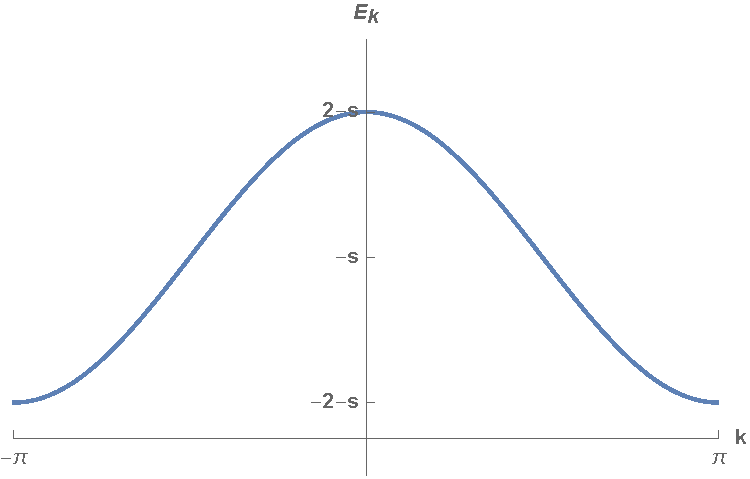
\includegraphics[width=1.0\textwidth]{HLTemplattBand}\\(a)
            \end{center}\end{minipage}
            \begin{minipage}[c]{0.3\textwidth}\begin{center}
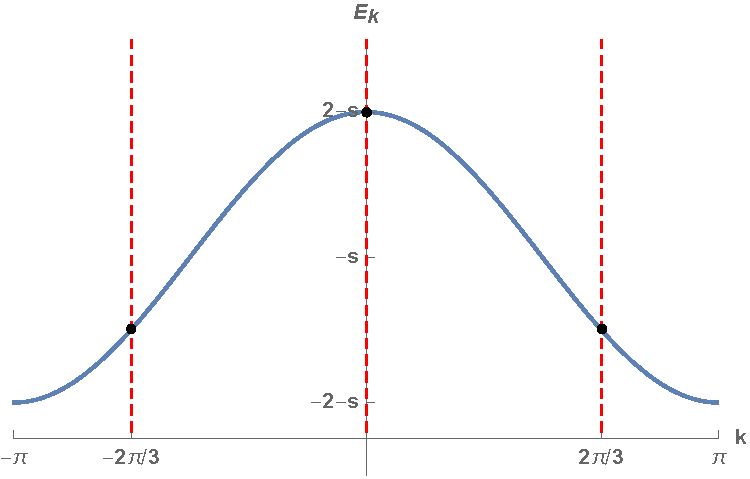
\includegraphics[width=1.0\textwidth]{HLTemplattBand3cycle}\\(b)
            \end{center}\end{minipage}
            \begin{minipage}[c]{0.3\textwidth}\begin{center}
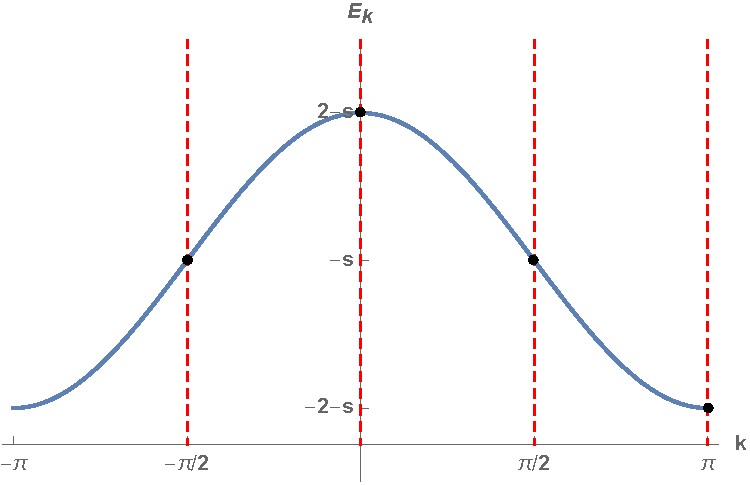
\includegraphics[width=1.0\textwidth]{HLTemplattBand4cycle}\\(c)
            \end{center}\end{minipage}
\end{center}
  \caption{\label{fig:LC21emplattBand}
(a) The eigenvalue $E_k$ of the \jacobianOrb\ on the infinite lattice as a function of the wave
vector $k$ in the first Brillouin zone. The \jacobianOrb\ has the reflection symmetry so the
eigenvalue is also invariant under the reflection $k\to -k$.
(b) For period 3 lattice states, the wave vectors of the eigenstates exist on the reciprocal lattice
spanned by $2\pi/3$. These lattice sites are labeled by the red dashed lines. There are only
3 period 3 eigenstates, with eigenvalues $s+1$, $s-2$ and $s+1$.
(c) For period 4 lattice states, the wave vectors of the eigenstates exist on the reciprocal lattice
spanned by $\pi/2$. These lattice sites are labeled by the red dashed lines. There are only
4 period 4 eigenstates, with eigenvalues $s$, $s-2$, $s$ and $s+2$.
$k=\pi$ and $k=-\pi$ are different by a reciprocal lattice translation, so they are a same
wave vector and should be only counted once.
          }
\end{figure}
%%%%%%%%%%%%%%%%%%%%%%%%%%%%%%%%%%%%%%%%%%%%%%%

Explain \reffig{fig:LC21emplattBand}.

        \PC{2021-09-02} {
I think I prefer some version of the identity \refeq{TableOfISP13952},
\refeq{HillDetOrbJ},
no mention of Chebyshev polynomials. Not important, will revisit later.
    }

% siminos/reversal/zeta1d.tex      pdflatex LC21; bibtex LC21
% temporary: siminos/spatiotemp/chapter/LC21zeta1d.tex
% $Author: predrag $ $Date: 2021-12-24 01:25:20 -0500 (Fri, 24 Dec 2021) $

%%%%%%%%%%%%%%%%%%%%%%%%%%%%%%%%%%%%%%%%%%%%%%%%%%%%
\begin{table}
\begin{tabular}{c|rrrrr|rrrrr|rrrrr}
$\cl{}$ &  1 &  2 &  3 &  4 &  5 &
       6 &  7 &  8 &  9 & 10 &
      11 \\%& 12 & 13 & 14 & 15 \\
\hline
$N_\cl{}$ &  2 &  4 &  8 & 16 &  32 &
       64 &  128 &  256 & 512 & 1024 &
      . % \\%& 12 & 13 & 14 & 15 \\
             \rule[-1ex]{0ex}{3.5ex} \\
$M_\cl{}$ &   2 &   1 &   2 &  3 &  6 &
         9 & 18 &  30 & 56  & 99 &
       186 &  %% &     &     &
\end{tabular}
\bigskip
\caption{\label{tab:LC21HamHenon}
{\Lattstate}s and %{prime}
orbit counts for the ${a}=6$ {\HenonMap}.
}
\end{table}
%%%%%%%%%%%%%%%%%%%%%%%%%%%%%%%%%%%%%%%%%%%%%%%%%%%%
%

\subsection{\Po\ theory}
\label{s:PoThe}

How come that a `$\Det$' in \refeq{fundFact} counts {\lattstate}s?

For a general, nonlinear fixed point condition $F[\Xx]=0$, expansion
\refeq{LnDet=TrLn2} in terms of traces is a cycle
expansion\rf{inv,AACI,ChaosBook}, with support on \emph{periodic orbits}.
Ozorio de Almeida and Hannay\rf{OzoHan84} were the first to relate the
number of periodic points to a \JacobianM\ generated volume; in 1984 they
used such relation as an illustration of their `principle of uniformity':
``periodic points of an ergodic system, counted with their natural
weighting, are uniformly dense in phase space.'' In \po\
theory\rf{inv,CBgetused} this principle is stated as a
\HREF{http://chaosbook.org/chapters/ChaosBook.pdf\#section.27.4} {flow
conservation} sum rule, where the sum is over all {\lattstate}s $\Mm$ of
period $\cl{}$,
\beq
\sum_{|\Mm|=\cl{}}
    \frac{1}{|\det (\id - \jMat_\Mm)|}
    \;= 1
\,,
\label{H-OdeA_mapsOrb}
\eeq
or, by Hill's formula \refeq{detDet},
\beq
\sum_{|\Mm|=\cl{}}
%\sum_{\ssp_i{\in\mbox{\footnotesize Fix}\map^{\cl{}}}}
    \frac{1}{|\Det\jMorb_\Mm|}
    \;=1
\,.
\label{Det(jMorb)eights}
\eeq
For the Bernoulli system the `natural weighting' takes a particularly
simple form, as the {\HillDet} of the {\jacobianOrb} is the same for all
periodic points of period $\cl{}$, $\Det\jMorb_\Mm=\Det\jMorb$, whose
number is thus given by \refeq{LC21detBern}.
For example, the sum over the $\cl{}=2$ {\lattstate}s is,
\beq
      \frac{1}{|\Det{\color{green}\jMorb_{00}}|}
   +    \frac{1}{|\Det{\color{red}\jMorb_{01}}|}
   + \frac{1}{|\Det{\color{yellow}\jMorb_{10}}|}
    =1
\,,
\ee{H-OdeA_mapsOrb2}
see \reffig{fig:BernCyc2Jacob}\,(b).
Furthermore, for any piece-wise
linear system all curvature corrections\rf{CBcount} for orbits of
periods $k>\cl{}$ vanish, leading to explicit {\lattstate}-counting
formulas of kind reported in this paper.

In the case of temporal Bernoulli or \templatt, the hyperbolicity is the same
everywhere and does not depend on a particular solution $\Xx_p$, counting
\po s is all that is needed to solve a cat-map dynamical system
completely; once \po s are counted, all {\cycForm s}\rf{CBtrace} follow.

This is the `\po\ theory'. And if you don't know,
\HREF{https://www.youtube.com/watch?v=_JZom_gVfuw} {now you know}.


\subsection{Remarks}
\label{s:LC21HillForm}

A succinct  explanation of the Hill's formula:
\begin{quote}
If you evaluate stability of the 3-term recurrence \refeq{JiKoKr20(2)} on
a periodic lattice you get the {\jacobianOrb} $\jMorb$;
if you evaluate it by multiplying the `two-configuration representation'
matrix $\jMps$, you get the `time evolution' side of the Hill's formula.
\end{quote}

The reformulation of the \catlatt\ 3-term recurrence
\refeq{catMapNewt} % {CatMap2dHill}
as the `two-configuration' map
\refeq{LC21PerViv} % {PV2config}
is a passage from the Lagrangian to the Hamiltonian formulation, also
known as `transfer matrix' formulation of lattice field
theories\rf{MonMun94,MunWal00} and Ising
models\rf{Onsager44,Kastening02}. We chose to prove it here using only
elementary linear algebra, not only because the Lagrangian
formalism\rf{BolTre10} is not needed for the problem at hand, but because
it actually obscures the generality of Hill's formula, which works
equally well for dissipative systems, such as the Bernoulli Hill's formula
\refeq{LC21PerViv}).

For Hamiltonian evolution \refeq{catMap}, the $[2\!\times\!2]$
\jacobianM\ $\jMat^\cl{}$ (the monodromy matrix of a \po) describes
the growth of an initial state perturbation in $\cl{}$ steps. For the
corresponding Lagrangian system with action $\action$,
% (see \refsect{s:catLagrForm}),
the first variation of
the action $\delta\action=0$ yields the Euler–Lagrange equations
\refeqs{LC21eqMotion}{catTempLatt}, while the second variation, the
$[\cl{}\!\times\!\cl{}]$ {\jacobianOrb} \refeq{tempCatFix},
describes the stability of the \emph{entire} given \po. In this,
classical mechanics context, Bolotin and Treschev\rf{BolTre10} refer to
$\jMorb$ as the `Hessian operator', but, as it is clear from our
Bernoulli discussion of \refsect{s:JacobianOrb}, and applications to \KS\
and Navier-Stokes systems\rf{GuBuCv17}, this notion of global stability
of orbits is general, and applies to all dynamical systems, not only the
Hamiltonian ones.

In preparing this section we have found expositions of Lagrangian
dynamics for discrete time systems by MacKay, Meiss and
Percival\rf{MKMP84,meiss92}, and Li and Tomsovic\rf{LiTom17b} particulary
helpful.
Hill's formula as derived by Mackay and Meiss\rf{MacMei83} and
Allroth\rf{Allroth83} (Allroth eq.~(12)) applies to
`one-degree-of-freedom' systems, \ie, 1D lattices with only the nearest
neighbor interactions. For a finite set of neighbors,
Allroth\rf{Allroth83} has partial results in the
context of Frenkel-Kontorova models.

Discrete Hill's formula plays important role in the theory of Toda
lattices\rf{Toda89}, \ie, classical mechanics of one-dimensional lattices
(chains) of particles with nearest neighbor interaction, discrete and
infinite in space, continuous in time.

The {\em inverse scattering method} for periodic systems this gives a
discrete Hill's equation, and in place of the scattering data, it is
convenient to use the spectrum of the discrete Hill's equation.
